\begin{frame}
	\frametitle{RA y RA en entornos universitarios}
	\block{\it Realidad Aumentada (RA)}
		\begin{itemize}
			\item {\it ¿Qué es la RA?}.
			\item {\it ¿Cómo funciona esta tecnología?}.
			\item {\it ¿Qué tipos de Realidad Aumentada existen?}.
			\item {\it ¿Diferencias entre la Realidad Aumentada y la Realidad Virtual (RV)?}.
			\item {\it ¿Qué es la Realidad Mixta?}.
			\item {\it Integración de la RA en Android Studio}.
		\end{itemize}
	\endblock{}
\end{frame}

%------------------------------------------------------------------

\begin{frame}
	\frametitle{RA}
		\block{\it ¿Qué es la realidad aumentada?}
		\begin{itemize}
			\item Permite expandir la información del mundo físico.
			\item Se encuentra en su mejor momento.
			\item Aplicaciones para todos los ámbitos. 
		\end{itemize}
		\endblock{}

		\begin{center}
			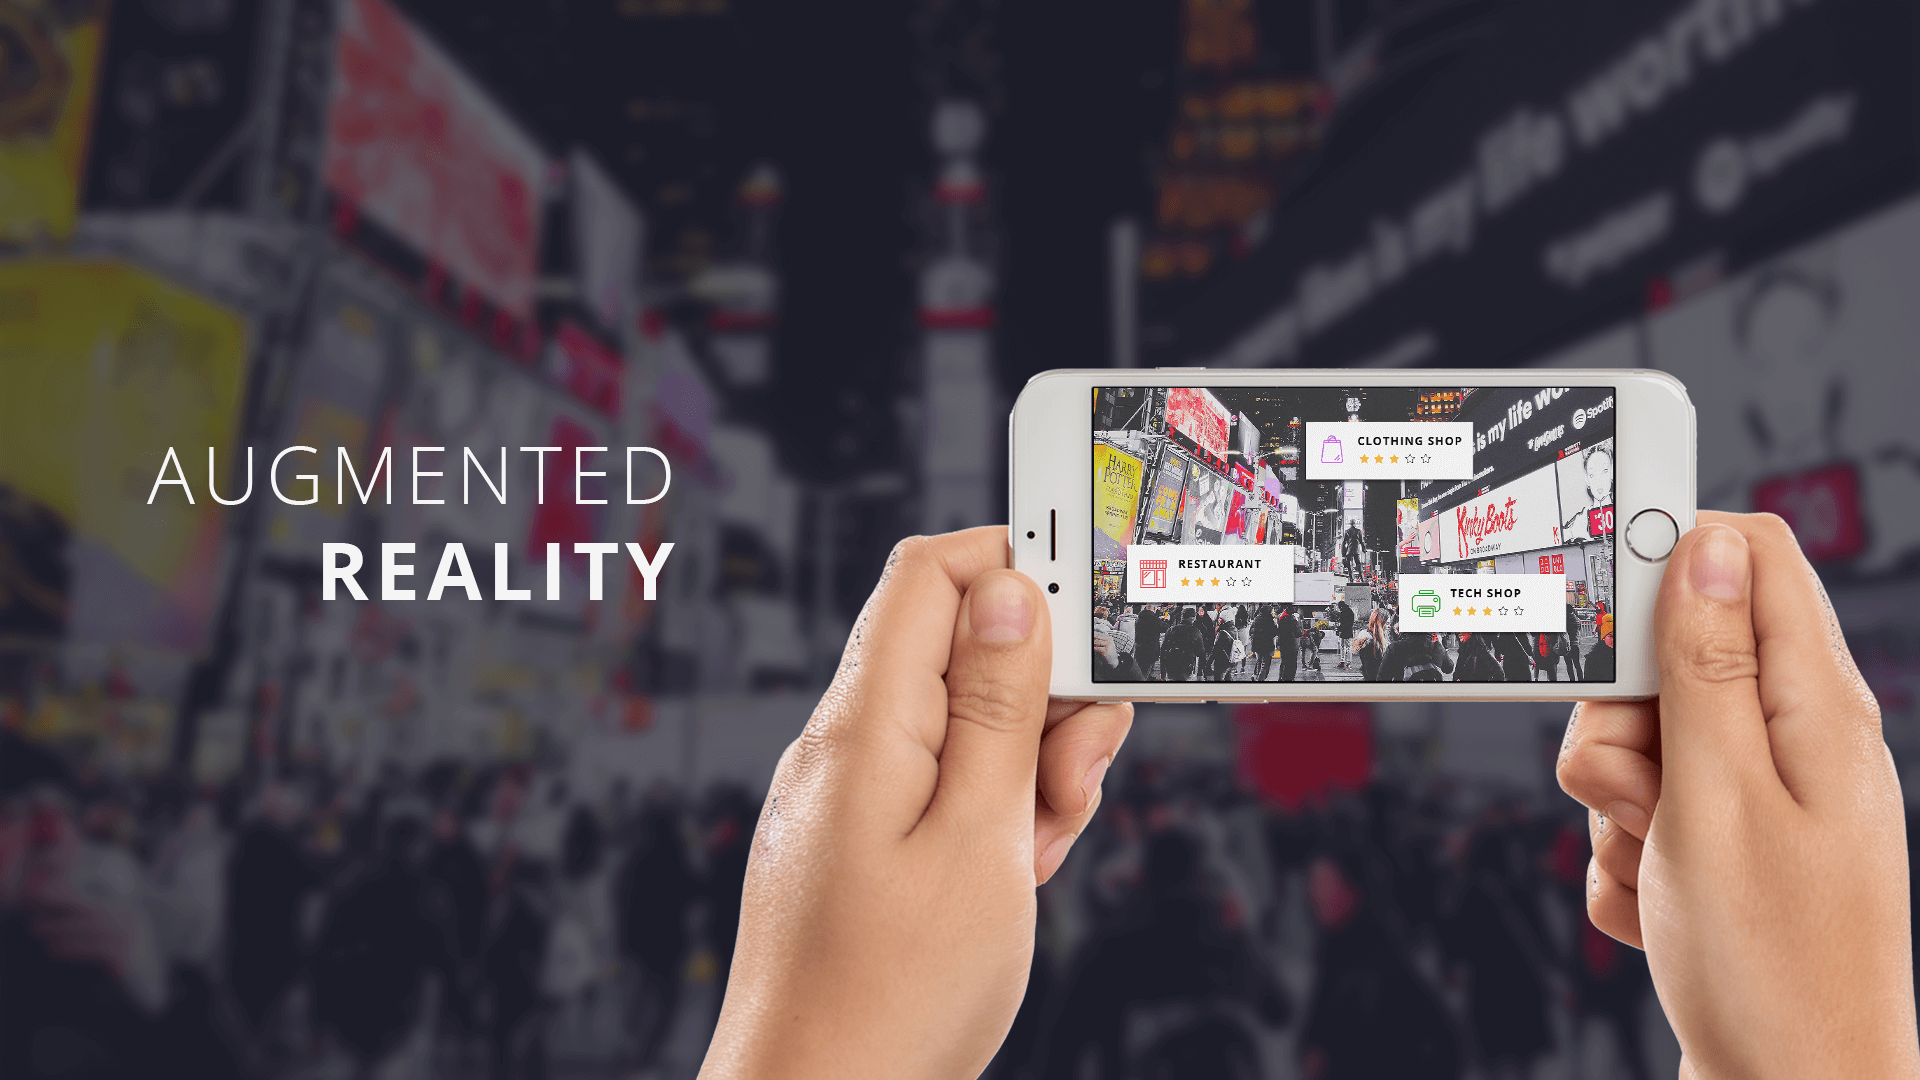
\includegraphics[width=0.7\linewidth]{Images/ar3}
		\end{center}
	
\end{frame}

%------------------------------------------------------------------
\begin{frame}
	\frametitle{RA}
		\block{\it ¿Cómo funciona esta tecnología?}
			Componentes necesarios para la tecnología de RA:
			\begin{itemize}
				\item {Dispositivo de visualización.}
				\item {Sistema de computación.}
				\item {Sensores: GPS, WIFI, Bluetooth, acelerómetro, giroscopio, cámara, etc.}
				\item {Software de RA.}
			\end{itemize}
		\endblock{}

		\begin{center}
			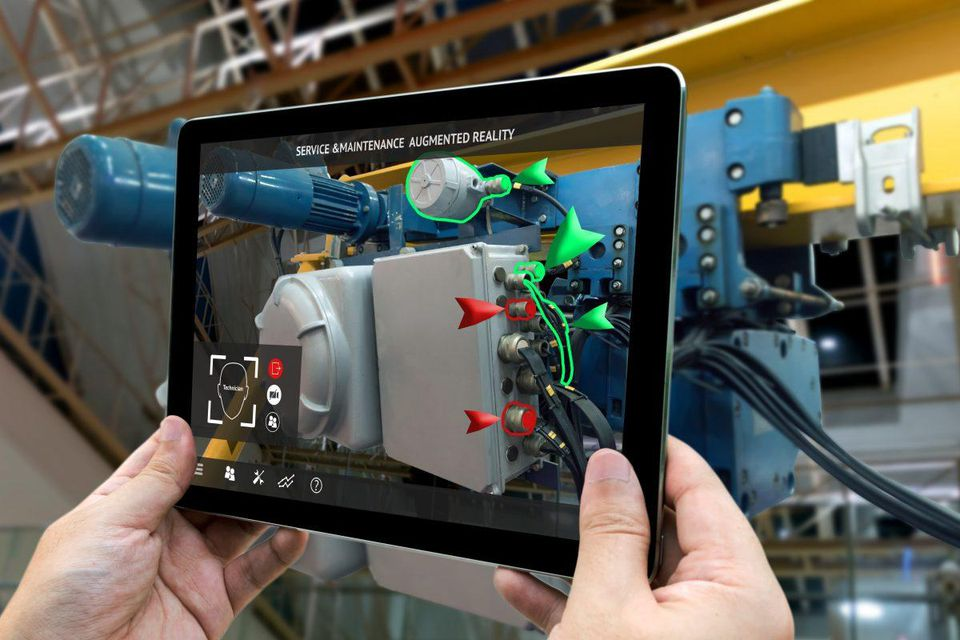
\includegraphics[width=0.43\linewidth]{Images/ar1}
		\end{center}
\end{frame}
		


\begin{frame}
	\frametitle{RA}
	\begin{columns}
			\begin{column}{0.45\textwidth}
				\block{\it ¿Qué tipos de RA existen?}
					Existen distintos tipos de RA:
					\begin{itemize}
						\item {Marker-based.}
						\item {Markerless.}
						\item {Pojection-based.}
						\item {Superimposition-based.}
					\end{itemize}
				\endblock{}
			\end{column}
			\begin{column}{0.55\textwidth}
				\vfill 
					\begin{center}
						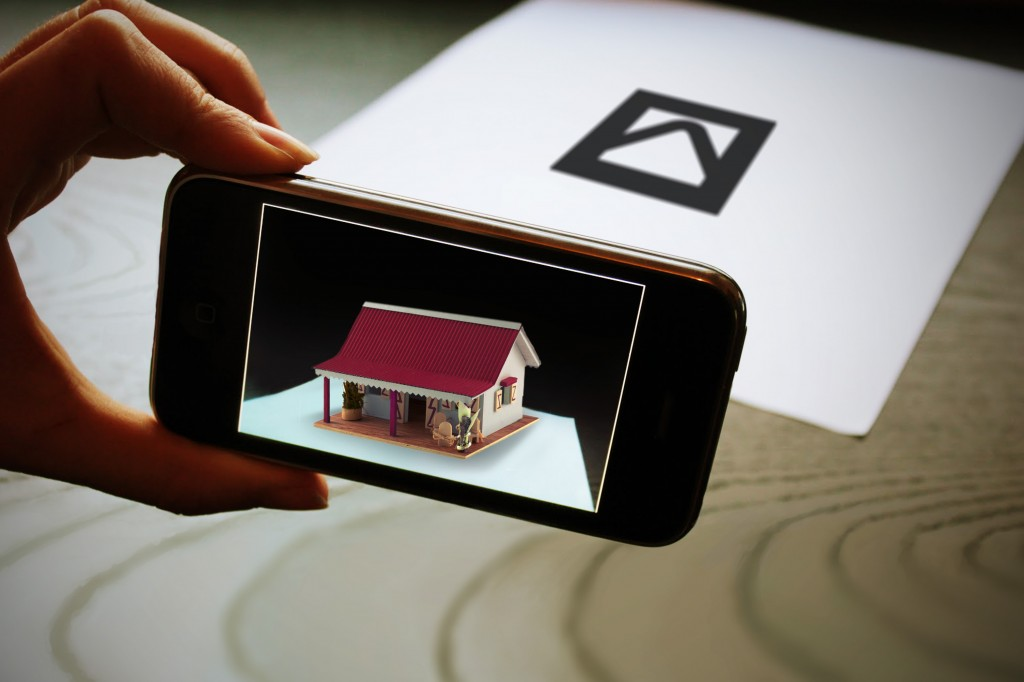
\includegraphics[width=0.95\linewidth]{Images/marker-ar}
					\end{center}
			\end{column}
	\end{columns}
\end{frame}

%------------------------------------------------------------------

\begin{frame}
	\frametitle{RA}
		\block{\it ¿Diferencias entre la Realidad Aumentada y la Realidad Virtual (RV)?}
			\begin{itemize}
				\item {En la actualidad se encuentra más avanzada que la RA.}
				\item {Muestra al usuario un entorno de escenas y objetos de aperiencia real.}
				\item {Dispone de distintos mecanismos de interacción.}
				\item {Aleja al usuario del entorno real.}
			\end{itemize}
		\endblock{}
			\begin{center}
				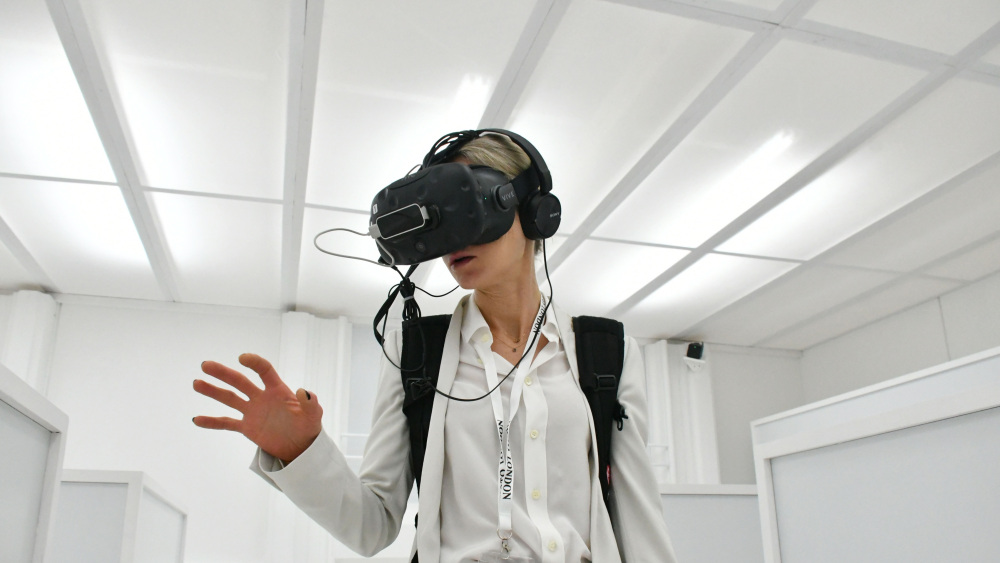
\includegraphics[width=0.50\linewidth]{Images/vr1}
			\end{center}
\end{frame}

%--------------------------------------------------------------------


\begin{frame}
	\frametitle{RA}
		\block{\it ¿Qué es la Realidad Mixta?}
			\begin{itemize}
				\item {Es la union de la RA con la RV}.
				\item {Consiste en llevar el mundo real al mundo virtual.}
				\item {Requiere de mayor capacidad de procesamiento que la RA.}
			\end{itemize}
		\endblock{}
		\vfill 
			\begin{center}
				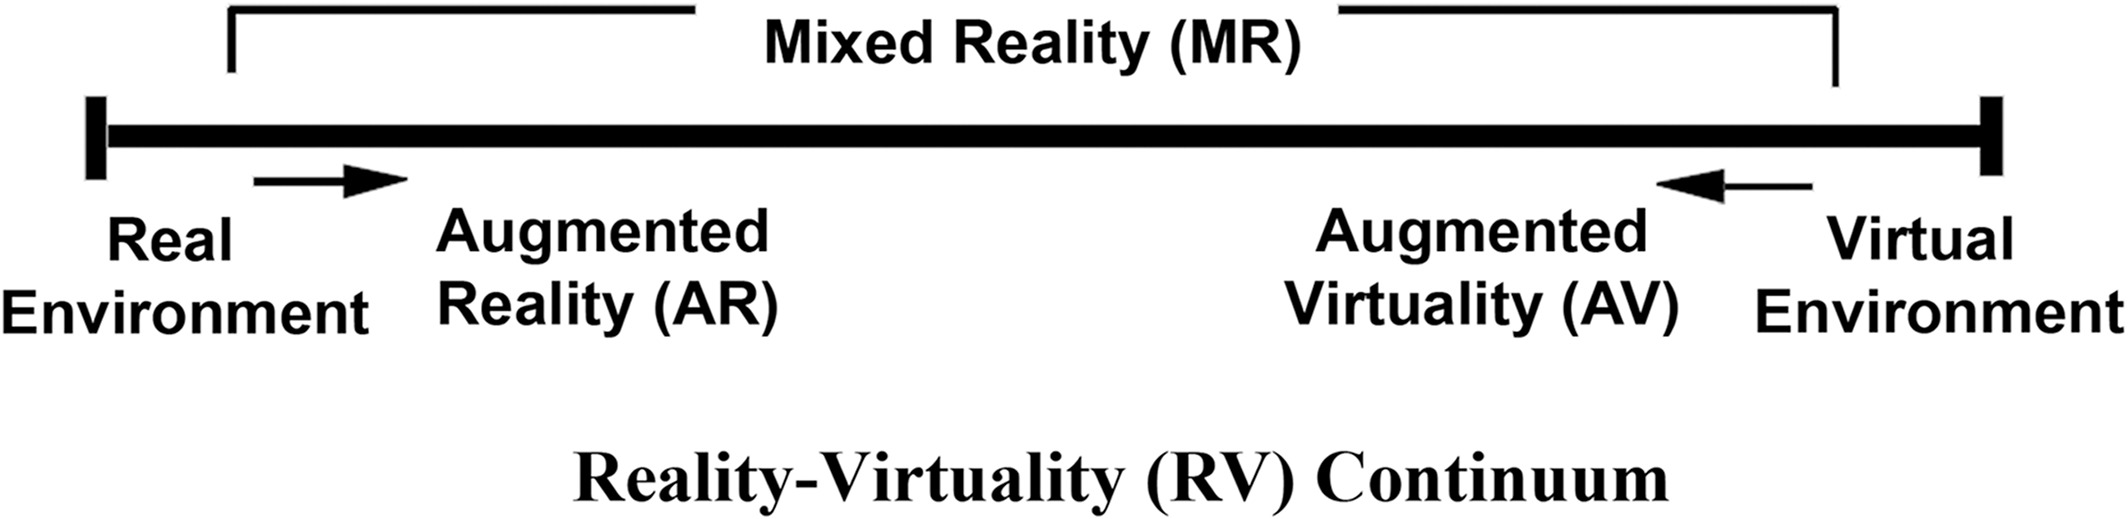
\includegraphics[width=0.8\linewidth]{Images/realidamixta}
			\end{center}
\end{frame}


\begin{frame}
	\frametitle{RA}
	\block{\it  Integración de la Realidad Aumentada en Android Studio}
		\begin{columns}
			\begin{column}{0.3\textwidth}
				\begin{center}					
					Vuforia 
				\end{center}
				\vspace{3mm}
				\vfill 
					\begin{center}
						
\includegraphics[width=0.8\linewidth]{Images/vuforia}
					\end{center}
			\end{column}
			\begin{column}{0.3\textwidth}
				\begin{center}
				Kudan AR SDK
				\end{center}
				\vspace{3mm}
				\vfill 
					\begin{center}
						
\includegraphics[width=0.8\linewidth]{Images/kudan}
					\end{center}
			\end{column}
			\begin{column}{0.3\textwidth}
				\begin{center}
					MaxST SDK
				\end{center}
				\vspace{3mm}
				\vfill 
					\begin{center}
						
\includegraphics[width=0.5\linewidth]{Images/maxst}
					\end{center}
			\end{column}
		\end{columns}
	\endblock{}
\end{frame}




\begin{frame}
	\frametitle{RA en entornos universitarios}
			\block{\it Aprendizaje}
				\begin{itemize}
					\item La RA se encuentra preparada para comenzar a acercarse a las aulas.
					\item Capacidad para generar material didactico y actividades para cualquier disciplina.
					\item Mejorar el aprendizaje.
					\item Experiencias mas ricas e inmersivas.
					\item Cambia la forma en la que adquieren los contenidos de aprendizaje.
				\end{itemize}
			\endblock{}
\end{frame}

%------------------------------------------------------------------

% \begin{frame}
% 	\frametitle{RA en entornos universitarios}
% 		\block{\it Beneficios principales}
% 			\begin{itemize}
% 				\item Aumentar o enriquecer la información de la realidad para hacerla más comprensible al alumno.
			
% 				\item El uso de una interfaz tangible para la manipulación de objetos, que permite observar un objeto desde diferentes puntos de vista,
% 				seleccionando, el discente, el momento y posición de observación.
			
% 				\item Potenciar el aprendizaje ubicuo.
				
% 				\item Crear escenarios ``artificiales'' seguros para el alumnado
% 				como pueden ser laboratorios o simuladores. 
			
% 				\item Enriquecer los materiales impresos para el alumnado con información adicional en diferentes soportes.
				
% 				\item Facilita la colaboración efectiva y discusión entre el alumnado.
% 			\end{itemize}
% 		\endblock{}
% \end{frame}


%---------------------------------------------------------------------

% \begin{frame}
% 	\frametitle{RA en entornos universitarios}
% 		\begin{columns}
% 			\begin{column}{0.6\textwidth}
% 				\block{\it Diseño de aplicaciones orientadas a la enseñanza}
% 				\begin{itemize}
% 					\item Ser sencillo y robusto.
% 					\item Permitir que el educador ingrese información de manera simple y efectiva.
% 					\item Proporcionar al alumno información clara y concisa.
% 					\item Permitir una fácil interacción entre estudiantes y educadores.
% 					\item Realizar procedimientos complejos transparentes para los alumnos.
% 					\item Ser rentable y fácilmente extensible.
% 				\end{itemize}
% 				\endblock{}
% 			\end{column}
% 			\begin{column}{0.4\textwidth}
% 				\vfill 
% 				\begin{center}
% 					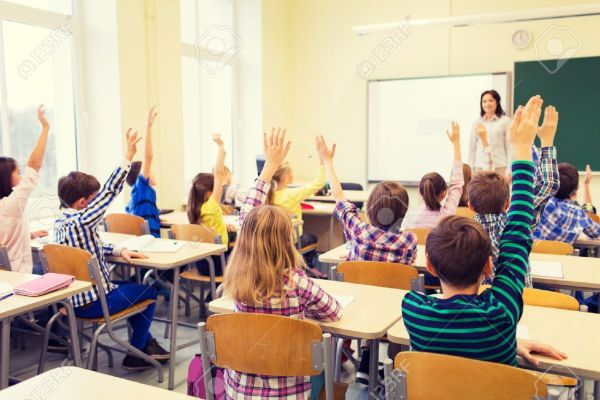
\includegraphics[width=0.9\linewidth]{Images/clase}
% 				\end{center}
% 			\end{column}		
% 		\end{columns}
% \end{frame}



\begin{frame}
	\frametitle{RA en entornos universitarios}
		\block{\it Aplicaciones en entornos universitarios}
			\begin{itemize}
				\item Prácticas en laboratorios.
			
				\item Practicas de campo y visitas.
			
				\item Libros y documentos.
				
				\item Aprendizajes experimentales.
			
				\item Información sobre la universidad.
				
			\end{itemize}
		\endblock{}
\end{frame}

